% GNUPLOT: LaTeX picture with Postscript
\begingroup
  \makeatletter
  \providecommand\color[2][]{%
    \GenericError{(gnuplot) \space\space\space\@spaces}{%
      Package color not loaded in conjunction with
      terminal option `colourtext'%
    }{See the gnuplot documentation for explanation.%
    }{Either use 'blacktext' in gnuplot or load the package
      color.sty in LaTeX.}%
    \renewcommand\color[2][]{}%
  }%
  \providecommand\includegraphics[2][]{%
    \GenericError{(gnuplot) \space\space\space\@spaces}{%
      Package graphicx or graphics not loaded%
    }{See the gnuplot documentation for explanation.%
    }{The gnuplot epslatex terminal needs graphicx.sty or graphics.sty.}%
    \renewcommand\includegraphics[2][]{}%
  }%
  \providecommand\rotatebox[2]{#2}%
  \@ifundefined{ifGPcolor}{%
    \newif\ifGPcolor
    \GPcolortrue
  }{}%
  \@ifundefined{ifGPblacktext}{%
    \newif\ifGPblacktext
    \GPblacktexttrue
  }{}%
  % define a \g@addto@macro without @ in the name:
  \let\gplgaddtomacro\g@addto@macro
  % define empty templates for all commands taking text:
  \gdef\gplbacktext{}%
  \gdef\gplfronttext{}%
  \makeatother
  \ifGPblacktext
    % no textcolor at all
    \def\colorrgb#1{}%
    \def\colorgray#1{}%
  \else
    % gray or color?
    \ifGPcolor
      \def\colorrgb#1{\color[rgb]{#1}}%
      \def\colorgray#1{\color[gray]{#1}}%
      \expandafter\def\csname LTw\endcsname{\color{white}}%
      \expandafter\def\csname LTb\endcsname{\color{black}}%
      \expandafter\def\csname LTa\endcsname{\color{black}}%
      \expandafter\def\csname LT0\endcsname{\color[rgb]{1,0,0}}%
      \expandafter\def\csname LT1\endcsname{\color[rgb]{0,1,0}}%
      \expandafter\def\csname LT2\endcsname{\color[rgb]{0,0,1}}%
      \expandafter\def\csname LT3\endcsname{\color[rgb]{1,0,1}}%
      \expandafter\def\csname LT4\endcsname{\color[rgb]{0,1,1}}%
      \expandafter\def\csname LT5\endcsname{\color[rgb]{1,1,0}}%
      \expandafter\def\csname LT6\endcsname{\color[rgb]{0,0,0}}%
      \expandafter\def\csname LT7\endcsname{\color[rgb]{1,0.3,0}}%
      \expandafter\def\csname LT8\endcsname{\color[rgb]{0.5,0.5,0.5}}%
    \else
      % gray
      \def\colorrgb#1{\color{black}}%
      \def\colorgray#1{\color[gray]{#1}}%
      \expandafter\def\csname LTw\endcsname{\color{white}}%
      \expandafter\def\csname LTb\endcsname{\color{black}}%
      \expandafter\def\csname LTa\endcsname{\color{black}}%
      \expandafter\def\csname LT0\endcsname{\color{black}}%
      \expandafter\def\csname LT1\endcsname{\color{black}}%
      \expandafter\def\csname LT2\endcsname{\color{black}}%
      \expandafter\def\csname LT3\endcsname{\color{black}}%
      \expandafter\def\csname LT4\endcsname{\color{black}}%
      \expandafter\def\csname LT5\endcsname{\color{black}}%
      \expandafter\def\csname LT6\endcsname{\color{black}}%
      \expandafter\def\csname LT7\endcsname{\color{black}}%
      \expandafter\def\csname LT8\endcsname{\color{black}}%
    \fi
  \fi
  \setlength{\unitlength}{0.0500bp}%
  \begin{picture}(7488.00,4464.00)%
    \gplgaddtomacro\gplbacktext{%
      \csname LTb\endcsname%
      \put(1474,704){\makebox(0,0)[r]{\strut{} 0}}%
      \put(1474,1109){\makebox(0,0)[r]{\strut{} 5e+06}}%
      \put(1474,1514){\makebox(0,0)[r]{\strut{} 1e+07}}%
      \put(1474,1919){\makebox(0,0)[r]{\strut{} 1.5e+07}}%
      \put(1474,2324){\makebox(0,0)[r]{\strut{} 2e+07}}%
      \put(1474,2729){\makebox(0,0)[r]{\strut{} 2.5e+07}}%
      \put(1474,3134){\makebox(0,0)[r]{\strut{} 3e+07}}%
      \put(1474,3539){\makebox(0,0)[r]{\strut{} 3.5e+07}}%
      \put(1606,484){\makebox(0,0){\strut{}$2^{8}$}}%
      \put(2099,484){\makebox(0,0){\strut{}$2^{10}$}}%
      \put(2592,484){\makebox(0,0){\strut{}$2^{12}$}}%
      \put(3085,484){\makebox(0,0){\strut{}$2^{14}$}}%
      \put(3579,484){\makebox(0,0){\strut{}$2^{16}$}}%
      \put(4072,484){\makebox(0,0){\strut{}$2^{18}$}}%
      \put(4565,484){\makebox(0,0){\strut{}$2^{20}$}}%
      \put(5058,484){\makebox(0,0){\strut{}$2^{22}$}}%
      \put(5551,484){\makebox(0,0){\strut{}$2^{24}$}}%
      \put(5683,704){\makebox(0,0)[l]{\strut{} 0}}%
      \put(5683,1177){\makebox(0,0)[l]{\strut{} 5e+07}}%
      \put(5683,1649){\makebox(0,0)[l]{\strut{} 1e+08}}%
      \put(5683,2122){\makebox(0,0)[l]{\strut{} 1.5e+08}}%
      \put(5683,2594){\makebox(0,0)[l]{\strut{} 2e+08}}%
      \put(5683,3067){\makebox(0,0)[l]{\strut{} 2.5e+08}}%
      \put(5683,3539){\makebox(0,0)[l]{\strut{} 3e+08}}%
      \put(176,2121){\rotatebox{-270}{\makebox(0,0){\strut{}Wall Time (microsec)}}}%
      \put(6980,2121){\rotatebox{-270}{\makebox(0,0){\strut{}Branch Misses}}}%
      \put(3578,154){\makebox(0,0){\strut{}Alphabet Size \small (log scale)}}%
    }%
    \gplgaddtomacro\gplfronttext{%
      \csname LTb\endcsname%
      \put(4696,4291){\makebox(0,0)[r]{\strut{}Wall Time, $mr\hat{\sigma}=$1.292 $avg\hat{\sigma}=$0.37}}%
      \csname LTb\endcsname%
      \put(4696,4071){\makebox(0,0)[r]{\strut{}Branch Miss, $mr\hat{\sigma}=$1.27 $avg\hat{\sigma}=$0.18}}%
    }%
    \gplbacktext
    \put(0,0){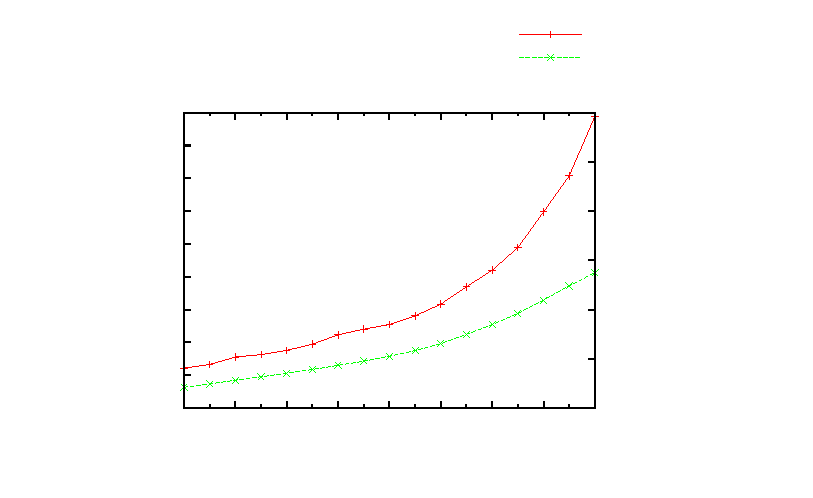
\includegraphics{naiveIntegerAlphabetSize_WallTime_BM}}%
    \gplfronttext
  \end{picture}%
\endgroup
